\begin{figure}
\centering
  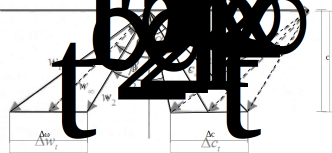
\includegraphics[width=\textwidth]{fig/SchiereCompr.pdf}
\caption{Schiere in movimento (compressore)}
\label{fig:SchiereCompr}
\end{figure}

\begin{figure}
\centering
  \includegraphics[width=\textwidth]{fig/ReticoloComp.pdf}
\caption{Reticolo di calcolo quasi-3D per un compressore assiale bistadio}
\label{fig:ReticoloComp}
\end{figure}

\begin{figure}
\centering
  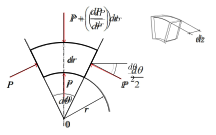
\includegraphics[width=\textwidth]{fig/concio.pdf}
\caption{Equilibrio radiale}
\label{fig:concio}
\end{figure}

\begin{figure}
\centering
  \includegraphics[width=\textwidth]{fig/VorticeLibero.pdf}
\caption{Pressione in funzione del raggio per un flusso a vortice libero}
\label{fig:VorticeLibero}
\end{figure}

\begin{figure}
\centering
  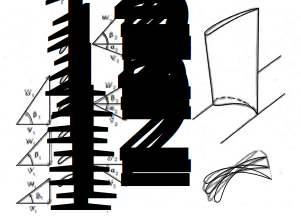
\includegraphics[width=\textwidth]{fig/TurboFan.pdf}
\caption{Profili e triangoli delle velocià per un rotore di turbo fan a vortice libero ($r_{TIP}/r_{HUB} =2$)}
\label{fig:TurboFan}
\end{figure}

\begin{figure}
\centering
  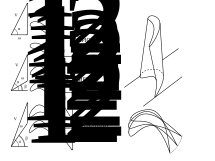
\includegraphics[width=\textwidth]{fig/TurbVortLib.pdf}
\caption{Profili e triangoli delle velocià per un rotore di uno stadio di bassa pressione di turbina a vapore o a gas ($r_{TIP}/r_{HUB} =1.4$)}
\label{fig:TurbVortLib}
\end{figure}



\begin{figure}
\centering
  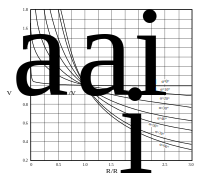
\includegraphics[width=\textwidth]{fig/AngPalCost.pdf}
\caption{}
\label{fig:AngPalCost}
\end{figure}

\begin{figure}
\centering
  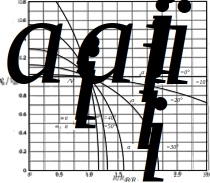
\includegraphics[width=\textwidth]{fig/VortForz.pdf}
\caption{Velocità assiale in funzione del raggio per un flusso a vortice forzato}
\label{fig:TurboFan}
\end{figure}


